\section{Pummping Lemma Kontextfrei}

Ein Codierungsverfahren verwendet die Zeichen $\Sigma$ = \{♣, ♢ , ♠ , ♡\} Aus technischen Gründen wird verlangt, dass die Anzahlen der verschiedenen Zeichen in einem Wort sich möglichst nicht unterscheiden, was exakt natürlich nur möglich ist, wenn die Wortlänge durch vier teilbar ist. Für zwei beliebige Zeichen $a,b \in \Sigma$ wird gefordert, dass \\
$$||W|_a - |w|_b| ≤ 1$$
die Anzahlen der Zeichen in einem Wort unterscheiden sich also höchstens um 1. Bei binärer Codierung ist diese Eigenschaft als DC-balance bekannt. Im binären Fall lässt sich DC-balance leicht mit einem Stackautomaten prüfen. Ist dies in diesem Fall mit vier Zeichen auch möglich? \\
$L = {w ∈ \Sigma^∗ | \ ||w|_a −|w|_b|≤ 1 ∀a,b ∈ \Sigma(a ≠ b)}$
1. Wir nehmen an, dass L kontextfrei ist. \\
2. Nach dem Pumping-Lemma für kontextfreie Sprachen gibt es eine Zahl N derart, dass Wörter $w ∈ L$ mit $|w|≥ N$ gepumpt werden.
3. Wir konstruieren das Wort $w = \{♣^N, ♢^N , ♠^N , ♡^N\}$
4. 
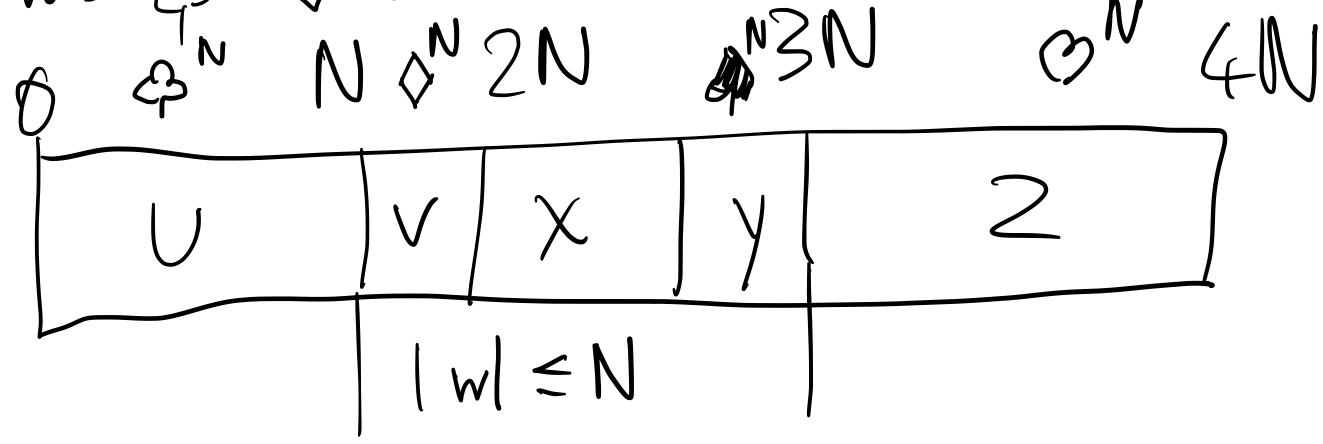
\includegraphics[width=\columnwidth]{img/kontexfreepump.png} \\
5. Beim Pumpen nimmt |♣|, |♢| zu nicht aber |♠| und |♡| $=>$ $ux^k xy^k z \in L | L \forall k ≠ 1$ \\
6. Widerspruch: L ist nicht kontextfrei

